% Homework Template
\documentclass[a4paper]{article}
\usepackage{ctex}
\usepackage{amsmath, amssymb, amsthm}
\usepackage{moreenum}
\usepackage{mathtools}
\usepackage{url}
\usepackage{bm}
\usepackage{enumitem}
\usepackage{graphicx}
\usepackage{subcaption}
\usepackage{booktabs}
\usepackage[mathcal]{eucal}
\usepackage[thehwcnt = 1]{iidef}
\usepackage {indentfirst}


\thecourseinstitute{清华大学电子工程系}
\thecoursename{\textbf{媒体与认知} \space 课堂2}
\theterm{2021-2022学年春季学期}
\hwname{作业}
\begin{document}

\courseheader
\name{郭中贺}
\vspace{3mm}
\centerline{\textbf{\Large{理论部分}}}

\section{单选题(15分)}
\subsection {\underline{B}}

\subsection {\underline{C}}

\subsection {\underline{A}}

\subsection {\underline{B}}

\subsection {\underline{B}}

\section{计算题(15 分)}

\begin{figure}[h]
    \centering
    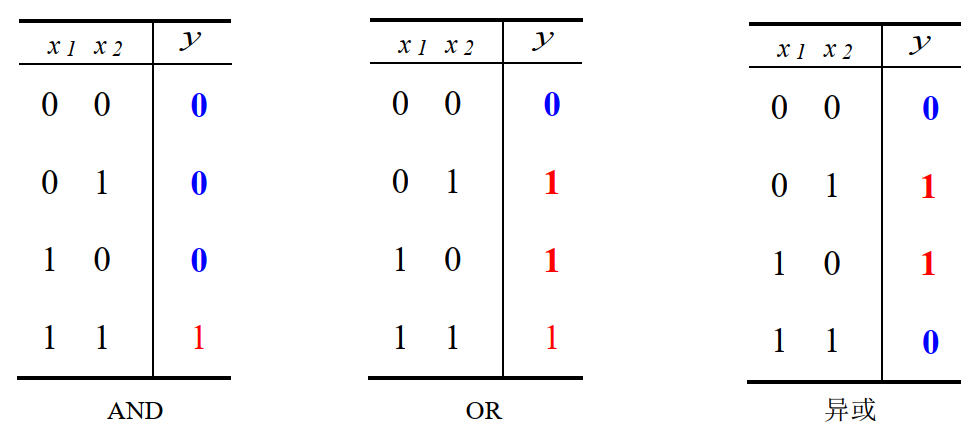
\includegraphics[width=12cm]{Fig1.png}
    \caption{AND,OR,异或三种逻辑运算}
    \label{fig:label_1}
\end{figure}

\subsection{基于如下单个人工神经元,设计实现两种逻辑门AND、OR运算。}
\setlength{\parindent}{2em}
\begin{equation}
    z=w_1x_1 +w_2x_2 + b
\end{equation}
\begin{equation}
y=f(z)=\left\{
        \begin{array}{l r}
        1, z > 0 \\
        0, z \leq 0
        \end{array}
\right.
\end{equation}
\subsubsection{AND实现}

只需取\[ w_1 = w_2 = 1, b = -1\]即可实现与门。\par
验证:只有当$x_1 = x_2 = 1$时,才能保证$z = x_1 + x_2 -1 = 1 > 0$,这样$y = 1$;当$x_1,x_2$中一个为1,另一个为0时,$z = x_1 + x_2 -1 = 0$,则$y = 0$;当$x_1=x_2=0$时,$z = x_1 + x_2 -1 = -1$,则$y = 0$。符合与门的设计。
\subsubsection{OR实现}
只需取\[ w_1 = w_2 = 1, b = 0\]即可实现或门。\par
验证:只有当$x_1 = x_2 = 0$时,才能保证$z = x_1 + x_2 +0 = 0$,这样$y = 0$;当$x_1,x_2$中一个为1,另一个为0时,$z = x_1 + x_2 + 0 = 1$,则$y = 1$;当$x_1=x_2=1$时,$z = x_1 + x_2 + 0 = 2$,则$y = 1$。符合或门的设计。
\subsection{上述形式的单个神经元是否可以实现逻辑门异或运算?如果是,请给出具体设计;若否,请解释理由。}
不可能实现,只需要根据异或门的要求列四个简单的不等式即可证明。
\[
b \leq 0,\quad
w_1 + b > 0,\quad
w_2 + b > 0,\quad
w_1 + w_2 + b \leq 0
\]
根据第二个和第三个式子,可得$$w_1 + w_2 + 2b > 0$$即\[ w_1 + w_2 + b > -b \geq  0 \]结合第四个式子可知\[ w_1 + w_2 + b  =  0 \]
再结合第二个和第三个式子可知,$w_1 < 0, w_2<0$,
结合第一个式子则有$w_1+w_2+b<0$,导出矛盾。因此上述形式的单个神经元不能实现异或运算。
\vspace{6mm}
\centerline{\textbf{\Large{编程部分}}}
\vspace{3mm}
% 请根据是否选择自选课题的情况选择“编程作业报告”或“自选课题开题报告”中的一项完成
\section{编程作业报告}
\subsection{训练模型}
运行 python classification.py train 训练模型后,
控制台输出结果与loss变化曲线分别如图2、3所示。其中图2的loss为对应训练轮数后的验证loss。\par
\begin{figure}[hp]
    \centering
    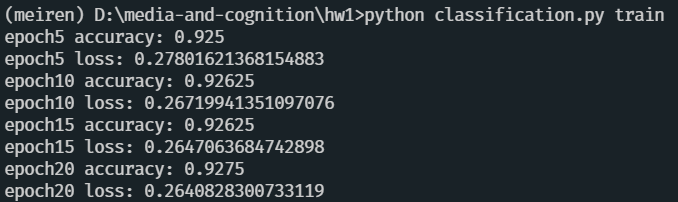
\includegraphics[width=8cm]{image/train_cmd.png}
    \caption{cmd输出结果}
\end{figure}
\begin{figure}[hp]
    \centering
    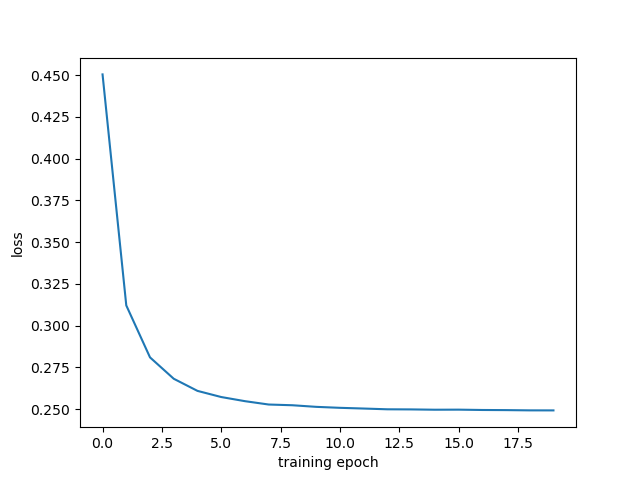
\includegraphics[width=8cm]{image/train_figure.png}
    \caption{loss曲线}
\end{figure}
结果分析:由图3曲线可知,一开始训练的loss较高,在0.5左右。
随着训练轮数的增加,loss逐渐下降,最终降到0.25左右。
另一方面,由图2输出,可知模型在验证集上的准确率较高,为92\% - 93\%,并且随着训练轮数增加
准确率有小幅度上升。可见该模型训练效果较好。
\subsection{测试模型}
运行 python classification.py test 验证模型,
控制台输出结果如图4所示。\par
\begin{figure}[hp]
    \centering
    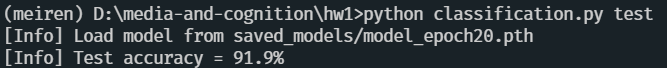
\includegraphics[width=8cm]{image/test_cmd.png}
    \caption{cmd输出结果}
\end{figure}
可见使用训练20轮之后的模型,在测试集上进行测试,其准确率也较高达到了91.8\%。
可见,该训练模型并不只能识别用于训练和验证的数据,具有一定的泛用性。
\subsection{可视化}
运行 python classification.py visual 进行可视化,
输出结果如图5所示。\par
\begin{figure}[hp]
    \centering
    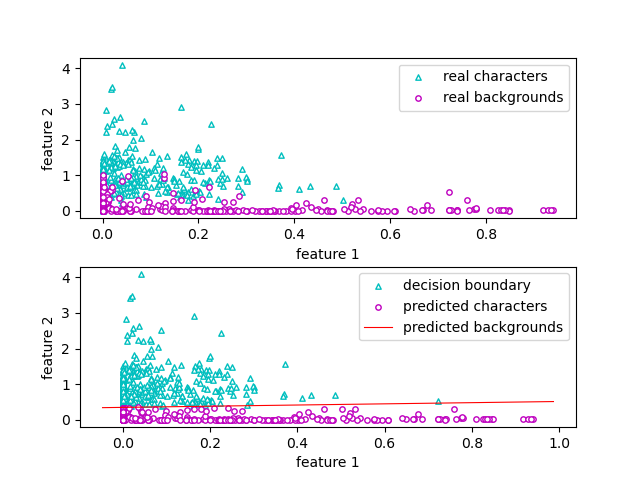
\includegraphics[width=10cm]{image/visual_figure.png}
    \caption{可视化结果}
\end{figure}
通过分析,我们可以看出:大部分的backgrounds
具有feature2数值较小的特点,且feature1分布较为分散。
而训练模型的decision boundary利用这一特点将characters和backgrounds进行分类。
大部分的数据能够分类正确。
\section{问题与解决}
本次编程作业较为简单,基本上按照助教习题课上的讲解
即可搭建一个线性分类器。难点主要在于自己编写二分类交叉熵函数以及不使用nn.Linear实现线性层。
二分类交叉熵函数由于其存在$\log$运算,因此如果遇到$\log 0 $则会导致计算出的loss均为inf出错。
我的解决方法是先将数据利用torch.clip()函数进行范围限制,防止出现$\log 0 $的情况,从而解决了这个问题。
另一方面,我使用nn.Parameter()自定义训练参数self.weight和self.bais,使得优化器能追踪这两个参数
并自动计算参数,forward函数利用torch.matmul()函数实现线性计算,实现了和nn.Linear()相同的功能。
\end{document}



%%% Local Variables:
%%% mode: late\rvx
%%% TeX-master: t
%%% End:
